
%***************************************************************************
%
% CreditCruncher - A portfolio credit risk valorator
% Copyright (C) 2004 Gerard Torrent
%
% This program is free software; you can redistribute it and/or
% modify it under the terms of the GNU General Public License
% as published by the Free Software Foundation; either version 2
% of the License.
%
% This program is distributed in the hope that it will be useful,
% but WITHOUT ANY WARRANTY; without even the implied warranty of
% MERCHANTABILITY or FITNESS FOR A PARTICULAR PURPOSE.  See the
% GNU General Public License for more details.
%
% You should have received a copy of the GNU General Public License
% along with this program; if not, write to the Free Software
% Foundation, Inc., 59 Temple Place - Suite 330, Boston, MA 02111-1307, USA.
%
%
% resolution.tex - TeX documentation file
% --------------------------------------------------------------------------
%
% 2005/01/22 - Gerard Torrent [gerard@fobos.generacio.com]
%   . initial release
%
%***************************************************************************

\chapter{Resoluci\'on}
\label{sec:resolution}

\section{Esquema general}

El m\'etodo de resoluci\'on implementado por CreditCruncher consiste en
aplicar el m\'etodo de Monte Carlo. En la figura \ref{fig:esquema1} se
muestra el esquema de un paso del m\'etodo de Monte Carlo.

\begin{figure}[!hb]
\begin{center}
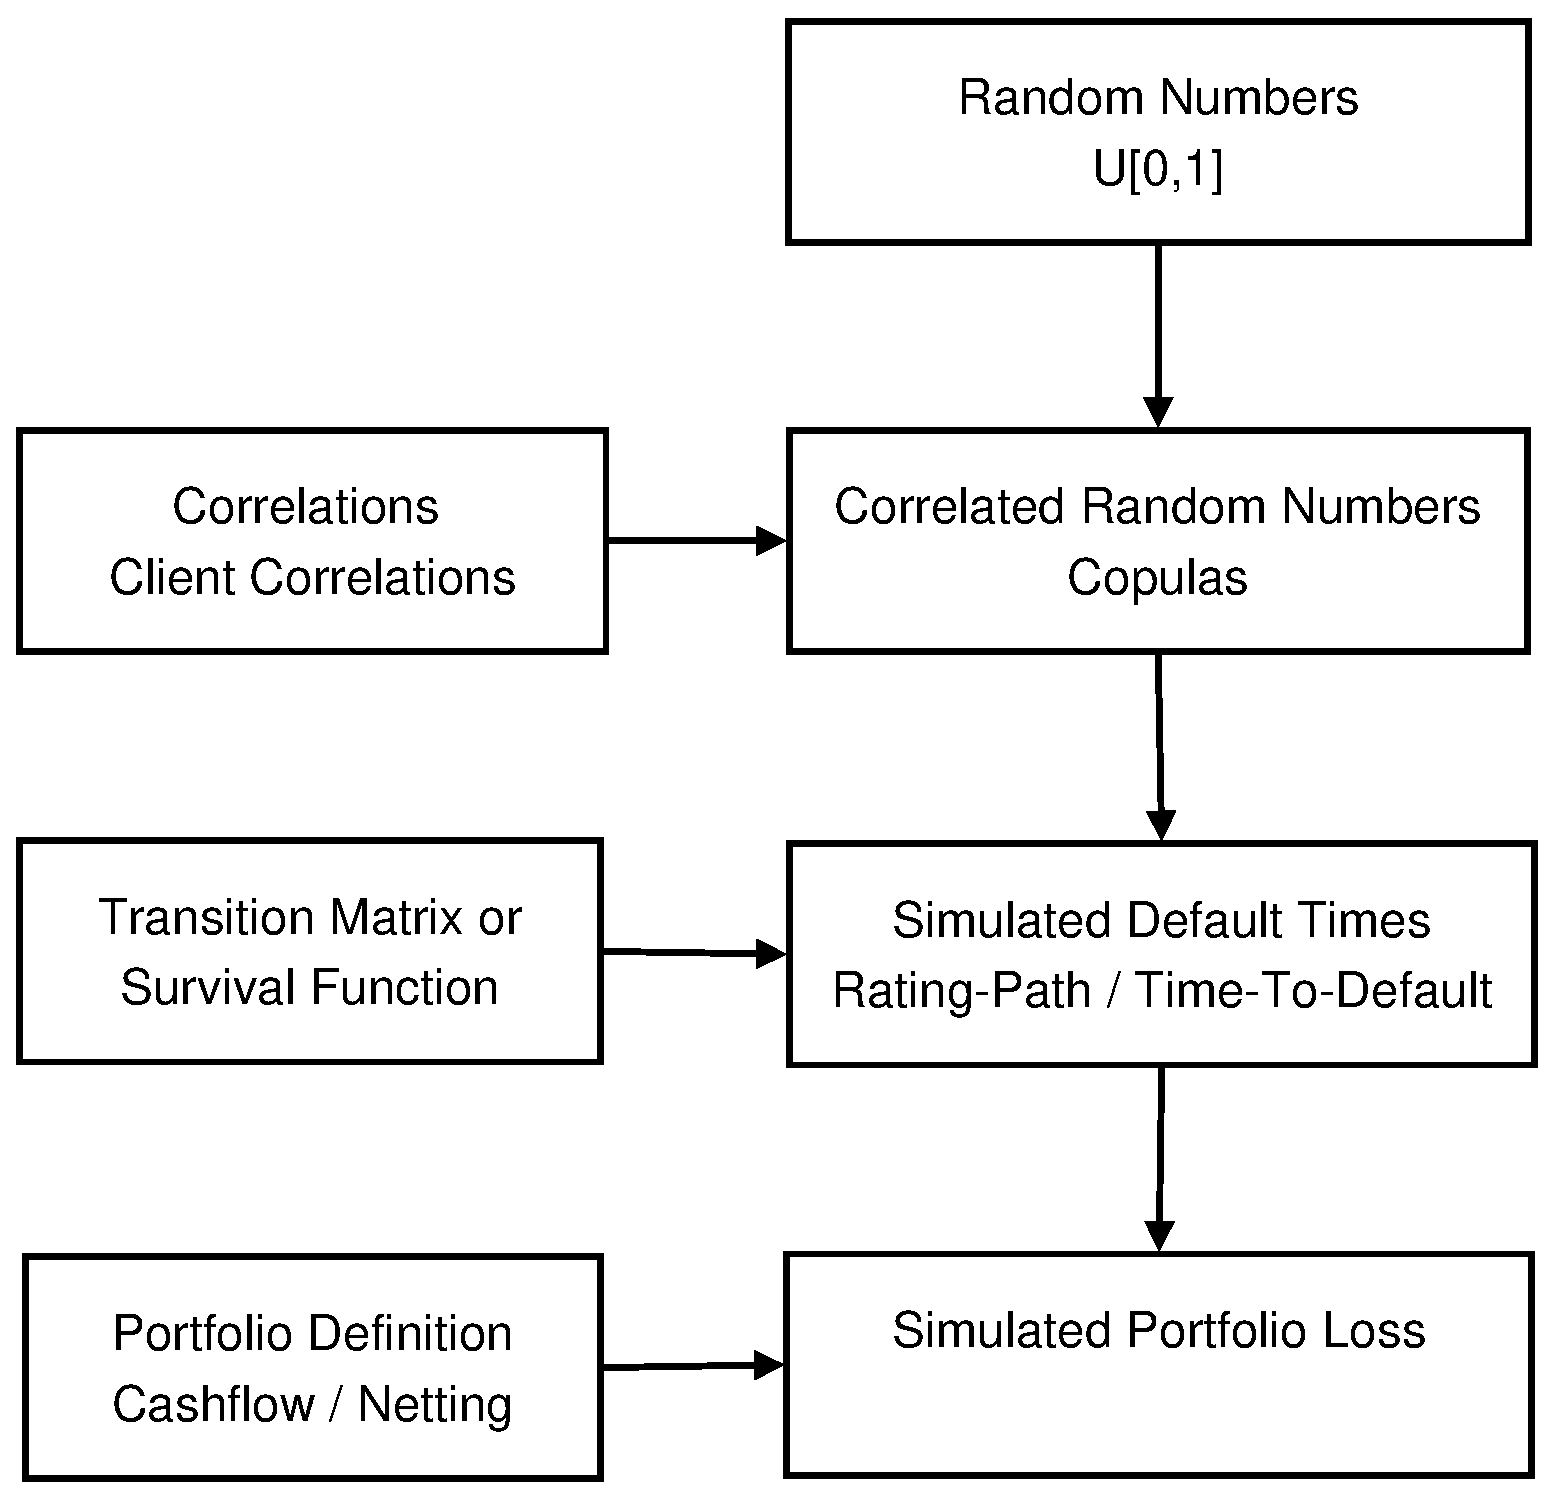
\includegraphics[width=10cm,angle=0]{./images/esquema1.eps}
\caption{Esquema de la simulaci\'on}
\label{fig:esquema1}
\end{center}
\end{figure}

%---------------------------------------------------------------------------

\section{El m\'etodo de Monte Carlo}

Se recomienda la lectura de la referencia \cite{mc:mervyn}. Se trata de los 
apuntes para una clase del profesor Mervyn Marasinghe. Se expone el m\'etodo 
de Monte Carlo y las t\'ecnicas de reducci\'on de la varianza.

\paragraph{Definici\'on.} Dado un conjunto de observaciones, $x_1, \cdots, x_N$,
de la variable aleatoria $X$, definimos la \emph{funci\'on de distribuci\'on emp\'irica}
\index{Funci\'on de distribuci\'on emp\'irica} como:
\begin{displaymath}
\widetilde{F_X(y)} = \frac{1}{N} \sum_{i=1}^{N} I_{(-\infty,y]}(x_i) \qquad
I_{(-\infty,y]}(x) = \left\{
\begin{array}{ll}
1 & \textrm{ if } x \in (-\infty,y] \cr
0 & \textrm{ otherwise}
\end{array}
\right.
\end{displaymath}

\paragraph{Proposici\'on.} La funci\'on de distribuci\'on emp\'irica tiende a 
la funci\'on de distribuci\'on al incrementar el n\'umero de observaciones.
\begin{displaymath}
\qquad \lim_{n\to\infty} \widetilde{F_X} = F_X
\end{displaymath}

\paragraph{Definici\'on.} Sea $X$ una variable aleatoria con funci\'on de 
distribuci\'on conocida, $F$. El \emph{m\'etodo de Monte Carlo}\index{M\'etodo
de Monte Carlo} consiste en obtener la funci\'on de distribuci\'on emp\'irica 
de la variable aleatoria $H(X)$ usando el siguiente m\'etodo:
\begin{displaymath}
\begin{array}{ccc}
F_X                 &     \quad       & \widetilde{F_{H(X)}}    \cr
\downarrow          &     \quad       & \uparrow                \cr
\textrm{simulation} &     \quad       & \textrm{empirical } cdf \cr
\downarrow          &     \quad       & \uparrow                \cr
x_1,\cdots,x_N      & \longrightarrow & H(x_1),\cdots,H(x_N)
\end{array}
\end{displaymath}

\paragraph{Observaci\'on.} Problemas aparentemente no relacionados con las 
variables aleatorias pueden reformularse como un problema donde intervenga
una variable aleatoria y ser resueltos por el m\'etodo de Monte Carlo. 
Normalmente se formula el problema original como el c\'alculo de un 
estad\'istico (pe. la media) sobre la funci\'on de distribuci\'on. Al
m\'etodo de Monte Carlo se le atribuye una velocidad de convergencia  
del orden de $1/\sqrt{N}$.

\paragraph{Ejemplo:} El ejemplo cl\'asico es obtener el valor de la integral 
de la funci\'on $W$ entre $0$ y $1$. Lo reformulamos de la siguiente forma:
\begin{displaymath}
\int_{0}^{1} W(u) du = \int_{0}^{1} W(u) \phi(u) du = E[W(U)]
\end{displaymath}
donde $U \sim U[0,1]$ y $\phi(u) = \textrm{pdf}(U) = 1$. La \'ultima igualdad se
establece usando la preposici\'on enunciada en el ap\'endice \ref{apendix:stats}.
Finalmente la integral se aproxima calculando la media de un conjunto de puntos
con distribuci\'on $W(U)$.

%---------------------------------------------------------------------------

\section{Variables aleatorias correlacionadas}

Se recomienda la lectura de las referencias \cite{copu:wang} y 
\cite{copu:pitfalls}. Se trata de art\'iculos donde se explica que es una 
c\'opula, sus propiedades, como simularlas, creencias err\'oneas, etc.

\paragraph{Definici\'on.} Llamamos \emph{c\'opula}\index{C\'opula} a la funci\'on
de distribuci\'on de una variable aleatoria $n$-dimensional tal que sus distribuciones
marginales \index{Distribuciones marginales} son variables aleatorias $U[0,1]$.
\begin{displaymath}
C(u_1, \cdots,u_n)=P(U_1 \leq u_1, \cdots, U_n \leq u_n) \qquad U_k \sim U[0,1]
\end{displaymath}

\begin{figure}[!hb]
\begin{minipage}[c]{0.5\columnwidth}%
  \centering
  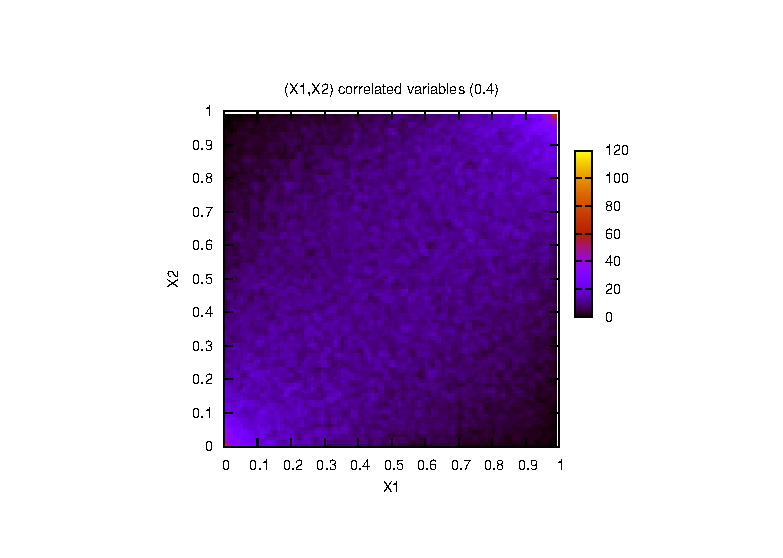
\includegraphics[height=5cm, angle=0]{./images/copula.eps}
\end{minipage}%
\hfill{}
\begin{minipage}[c]{0.5\columnwidth}%
  \centering
  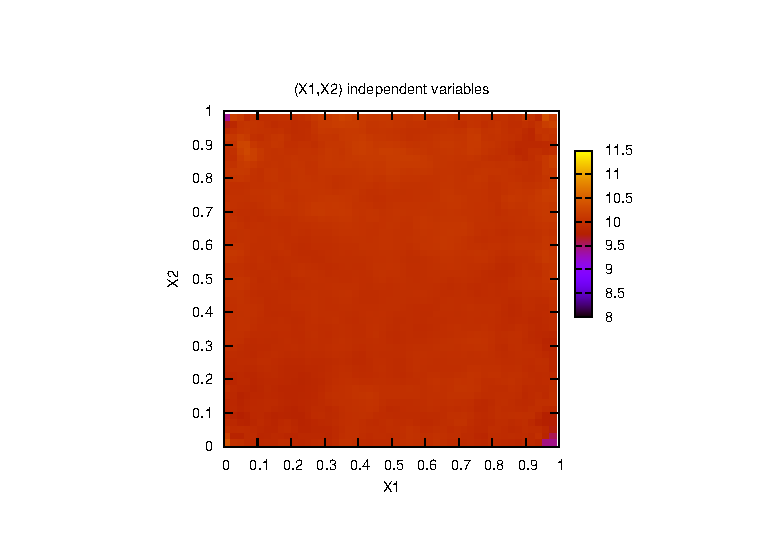
\includegraphics[height=5cm, angle=0]{./images/uniform.eps}
\end{minipage}%
\caption{Bivariate distribution plot with correlated and uncorrelated variables}
\label{copulas}
\end{figure}

\paragraph{Teorema.} \index{Teorema de Sklar} Toda variable aleatoria $n$-dimensional
puede separarse en las distribuciones seguidas por sus componentes (las distribuciones
marginales) y una c\'opula. Sea $F$ una funci\'on de distribuci\'on $n$-dimensional y
$f_1,\cdots, f_n$ sus marginales. El teorema de Sklar asegura que existe una 
c\'opula $C$ tq.
\begin{displaymath}
F(x_1, \cdots,x_n) = C(f_1(x_1), \cdots, f_n(x_n)) 
\end{displaymath}

\paragraph{Observaci\'on.} Una variable aleatoria $n$-dimensional no est\'a 
determinada por sus marginales y correlaciones entre estas. Dicho de otra
forma, existen infinitas formas de combinar las distribuciones marginales
 a trav\'es de c\'opulas de forma que cumplan las correlaciones. Las distribuciones 
el\'ipticas (que incluyen la distribuci\'on multinomial) son una excepci\'on. 

%---------------------------------------------------------------------------

\section{Simulaci\'on del tiempo de fallido}

El objetivo de este apartado es proporcionar m\'etodos para simular los
tiempos de fallido, $\vec{t_w} = (t_w^1,t_w^2,t_w^3,\cdots,t_w^{nc})$ de los
clientes cumpliendo:
\begin{itemize}
\item los fallidos de cada cliente deben satisfacer la matriz de transici\'on $M_T$
(o la funci\'on de supervivencia, $Survival(r,t)$).
\item la correlaci\'on entre los fallidos de los clientes debe cumplir la matriz
de correlaci\'on entre clientes, $\Theta$
\end{itemize}

\subsection{M\'etodo Rating-Path}
\label{res:mrt}
\index{M\'etodo Rating-Path}

Este m\'etodo simula la evoluci\'on del rating del cliente a lo largo del tiempo.
El tiempo de fallido se obtiene al alcanzar el rating $Default$. Para este m\'etodo
es necesario disponer de la matriz de transici\'on, $M_T$.

\paragraph{Paso 1.} Segmentamos el tiempo en intervalos constantes de forma que
el intervalo de tiempo entre $t_i$ y $t_{i+1}$ es el cubierto por la matriz de
transici\'on, $T$.
\begin{displaymath}
t_0,t_1,t_2,\cdots,t_k, \cdots
\end{displaymath}

\paragraph{Paso 2.} Para cada intervalo de tiempo $k$ creamos una c\'opula,
$Qk$ de dimensi\'on $nc$ que satisfaga la matriz de correlaci\'on entre
clientes, $\Theta$.
\begin{displaymath}
Q_1, Q_2, Q_3, \cdots, Q_k, \cdots
\end{displaymath}

\paragraph{Paso 3.} Simulamos las c\'opulas $Q_1, Q_2, Q_3, \cdots, Q_k, \cdots$.
Cada realizaci\'on de $Q_k$ consiste en un vector de componentes
$(Q_k(1), Q_k(2), \cdots, Q_k(nc))$.

\paragraph{Paso 4.} Simulamos el rating del cliente $i$ en $t_1$ de la forma siguiente:
disponemos del rating inicial $rating(i,t_0)$ y un valor $Q_1(i) \in [0,1]$
proporcionado por el componente $i$-\'esimo de $Q_1$. Entonces
\begin{displaymath}
rating(i,t_1) = M_T^{-1}(rating(i,t_1),Q_1(i))
\end{displaymath}
Este paso se encuentra ilustrado en la figura \ref{simrp}.

\paragraph{Paso 5.} Simulamos el rating del cliente $i$ en $t_k$ de la forma siguiente:
disponemos del rating anterior $rating(i,t_{k-1})$ y un valor $Q_k(i) \in [0,1]$
proporcionado por el componente $i$-\'esimo de $Q_k$. Entonces
\begin{displaymath}
rating(i,t_k) = M_T^{-1}(rating(i,t_{k-1}),Q_k(i))
\end{displaymath}
Este paso se encuentra ilustrado en la figura \ref{simrp}. Finalmente, aproximamos
el tiempo de fallido del cliente $i$ de la siguiente forma:
\begin{displaymath}
t_w^i = inf\{t_k | rating(i,t_k) = Default\}
\end{displaymath}

\begin{figure}[!hb]
\begin{center}
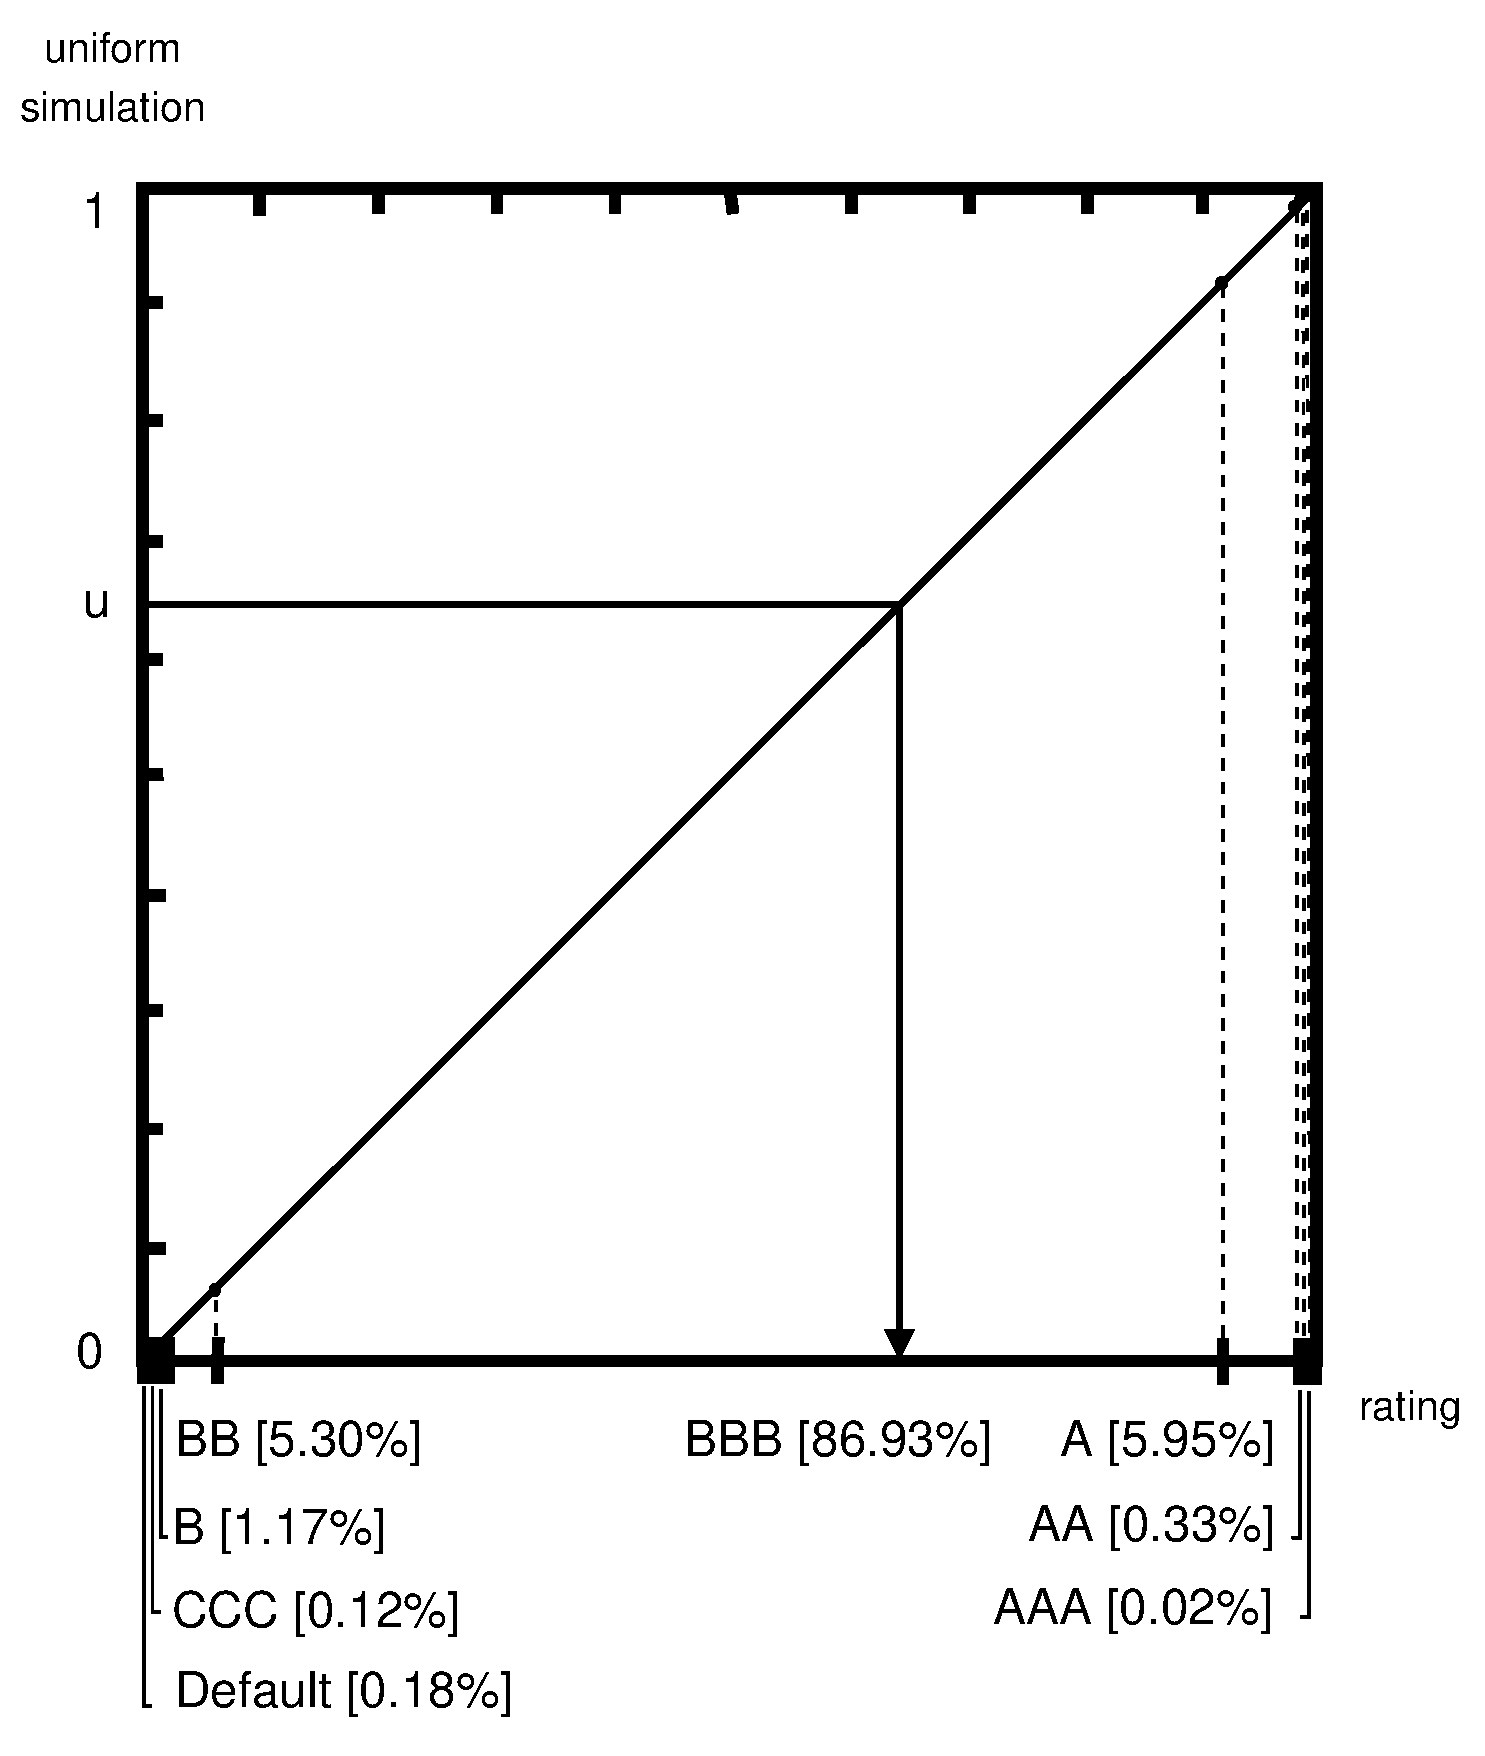
\includegraphics[width=7cm,angle=0]{./images/simrp.eps}
\caption{Simulaci\'on de la evoluci\'on del rating $BBB$ a $T$ tiempo}
\label{simrp}
\end{center}
\end{figure}

\subsection{M\'etodo Time-To-Default}
\label{res:mttd}
\index{M\'etodo Time-To-Default}

Este m\'etodo consiste en simular directamente el tiempo de fallido de los
clientes. Requiere disponer de la funci\'on de supervivencia. En caso
de disponer solamente de la matriz de transici\'on puede calcularse la funci\'on
de supervivencia asociada a la matriz de transici\'on usando las f\'ormulas
\ref{eq:survival1} y \ref{eq:cdfr1}.

\paragraph{Paso 1.} Creamos una c\'opula de dimensi\'on $nc$ que satisfaga la
matriz de correlaci\'on entre clientes, $\Theta$.
\begin{displaymath}
Q
\end{displaymath}

\paragraph{Paso 2.} Simulamos la c\'opula $Q$. La realizaci\'on de $Q$ consiste
en un vector de componentes $(Q(1), Q(2), \cdots, Q(nc))$.

\paragraph{Paso 2.} Simulamos el tiempo de fallido del cliente $i$ de la forma siguiente:
disponemos del rating inicial, $rating(i,t_0)$ y un valor $Q(i) \in [0,1]$ proporcionado
por el componente $i$-\'esimo de $Q$. Entonces:
\begin{displaymath}
t_w^i = Survival^{-1}(rating(i,t_0),Q(i))
\end{displaymath}
Este paso se encuentra ilustrado en la figura \ref{simttd}.

\begin{figure}[!hb]
\begin{center}
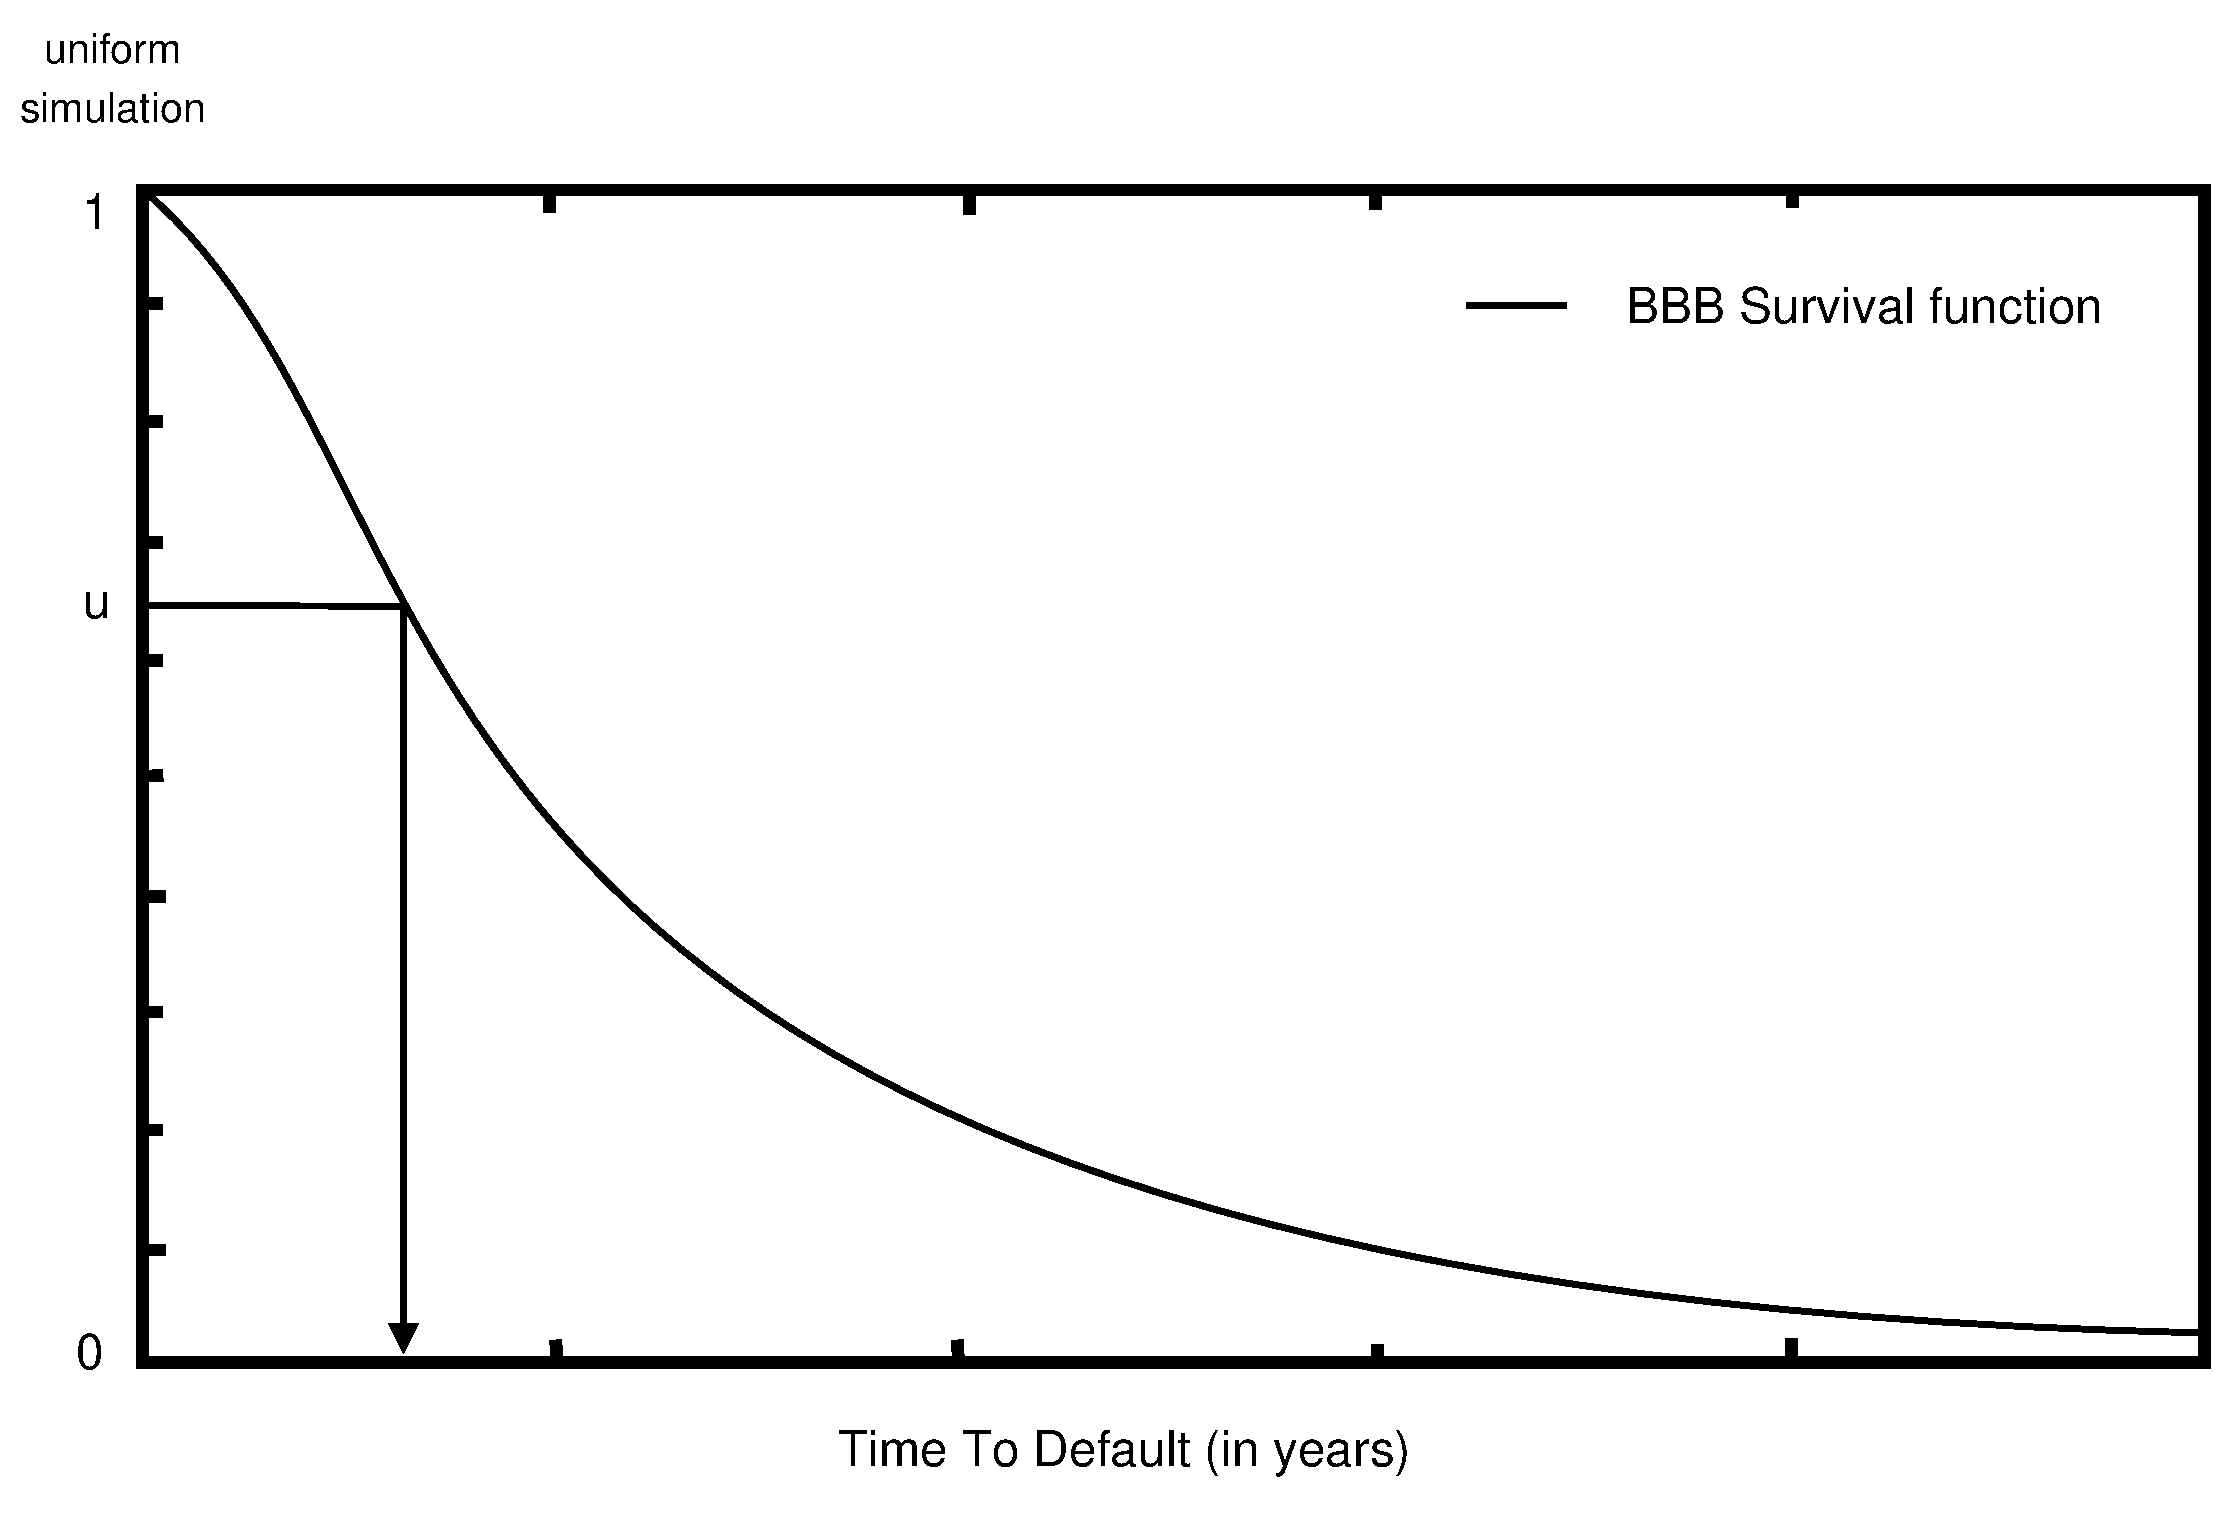
\includegraphics[width=10cm,angle=0]{./images/simttd.eps}
\caption{Simulaci\'on del tiempo hasta el fallido del rating $BBB$}
\label{simttd}
\end{center}
\end{figure}

%---------------------------------------------------------------------------

\section{Evaluaci\'on de la cartera}

En las definiciones siguientes se considera que $S$ es la curva spot en $t_0$,
$na_i$ es el n\'umero de activos del cliente $i$ y $nc$ el n\'umero de clientes.
Asimismo se considera que el casflow y netting de cada activo est\'a fijado y
no depende de la evoluci\'on del cliente.

\paragraph{Definici\'on.} Definimos el valor del activo $j$ del cliente $i$
evaluado en $t_K$ entre el tiempo $t_0$ y $t_K$, habiendo hecho fallido en
tiempo $t_w$ como:
\begin{equation}
X_{i,j}(t_w;t_0,t_K) = 
\end{equation}
\begin{displaymath}
\textrm{1}_{[t_w \leq t_K]} \cdot \textrm{netting}(t_w) \cdot \Upsilon_S(t_w,t_K) + 
\sum_{t=t_0}^{t_K} \textrm{1}_{[t < t_w]} \cdot \textrm{cashflow}(t) \cdot \Upsilon_S(t,t_K)
\end{displaymath}

\paragraph{Definici\'on.} Definimos el valor de los activos del cliente $i$
evaluados en $t_K$ entre el tiempo $t_0$ y $t_K$, habiendo hecho fallido en
tiempo $t_w$ como:
\begin{equation}
X_i(t_w;t_0,t_K) = \sum_{j=0}^{na_i} X_{i,j}(t_w;t_0,t_K)
\end{equation}

\paragraph{Definici\'on.} Definimos el valor de la cartera evaluada en $t_K$
entre el tiempo $t_0$ y $t_K$, siendo $\vec{t_w}$ los tiempos en los que han hecho
fallido los clientes como:
\begin{equation}
X(\vec{t_w};t_0,t_K) = \sum_{i=0}^{nc} X_i(t_w^i;t_0,t_K) =
\sum_{i=0}^{nc} \sum_{j=0}^{na_i} X_{i,j}(t_w^i;t_0,t_K)
\end{equation}

\paragraph{Definici\'on.} Definimos las p\'erdidas de la cartera evaluada en $t_K$
entre el tiempo $t_0$ y $t_K$, siendo $\vec{t_w}$ los tiempos en los que han hecho
fallido los clientes como:
\begin{equation}
Z(\vec{t_w};t_0,t_K) = X(\vec{t_\infty};t_0,t_K) - X(\vec{t_w};t_0,t_K)
\end{equation}

%---------------------------------------------------------------------------

\section{Valoraci\'on del riesgo}
\label{res:risk}

El m\'etodo de Monte Carlo genera $N$ realizaciones, $\{z_1,z_2,z_3,\cdots,z_N\}$,
de la variable aleatoria $Z$ (p\'erdidas de la cartera) que permiten obtener la
funci\'on de distribuci\'on emp\'irica. A continuaci\'on se exponen los estad\'isticos
calculados, sus estimaciones y el intervalo de confianza al nivel de confianza $\alpha$.
CreditCruncher utiliza el entorno \emph{R} \footnote{http://www.r-project.org} para realizar
los c\'alculos estad\'isticos. Para mas informaci\'on acerca de \emph{R} v\'ease \cite{stats:R}.
Sea $\phi^{-1}(x)$ la inversa de la funci\'on de distribuci\'on de la Normal(0,1).

\paragraph{Expected Loss.}\index{Expected Loss} F\'ormula extra\'ida de \cite{stats:schaum}
basada en el teorema del l\'imite central.
\begin{displaymath}
\mu_Z = \widehat{\mu_Z} \pm \phi^{-1}\left(\frac{1-\alpha}{2}\right) \cdot \frac{\widehat{\sigma_Z}}{\sqrt{N}}
\end{displaymath}
Consulte \ref{apendix:estim} para el c\'alculo de $\widehat{\mu_Z}$ y $\widehat{\sigma_Z}$.

\paragraph{Desviaci\'on est\'andar.}\index{Desviaci\'on Est\'andar} F\'ormula extra\'ida de
\cite{stats:schaum} basada en el teorema del l\'imite central.
\begin{displaymath}
\sigma_Z = \widehat{\sigma_Z} \pm \phi^{-1}\left(\frac{1-\alpha}{2}\right) \cdot \frac{\widehat{\sigma_Z}}{\sqrt{2N}}
\end{displaymath}
Consulte \ref{apendix:estim} para el c\'alculo de $\widehat{\sigma_Z}$.

\paragraph{Value at Risk.}\index{Value At Risk} Fijado un nivel de $VAR = x$
\begin{displaymath}
VAR_{x}(Z) = \widehat{q_{x}(Z)} \pm \phi^{-1}\left(\frac{1-\alpha}{2}\right) \cdot \textrm{stderr}(q_{x}(Z))
\end{displaymath}
Consulte \ref{apendix:estim} y \ref{apendix:stderrvar} para el c\'alculo de
$\widehat{q_{x}(Z)}$ y $\textrm{stderr}(q_{x}(Z))$.

\paragraph{TCE o Expected Shortfall.}\index{Tail Conditional Expectation}\index{Expected Shortfall}
Fijado un nivel de $VAR = x$
\begin{displaymath}
TCE_{x}(Z) = \widehat{TCE_{x}(Z)} \pm \phi^{-1}\left(\frac{1-\alpha}{2}\right) \cdot \textrm{stderr}(TCE_{x}(Z))
\end{displaymath}
Consulte \ref{apendix:estim} y \ref{apendix:stderrtce} para el c\'alculo de
$\widehat{TCE_{x}(Z)}$ y $\textrm{stderr}(TCE_{x}(Z))$.
